\documentclass[12pt]{zjutbook}

\zjuttype{本科毕业设计说明书(论文)}
\zjutyear{2022}
\zjuttitle{不得超过30个汉字,论文题目过长可分两行书写}
\zjutauthor{作者姓名}
\zjutmentor{教师姓名}
\zjutcollege{计算机科学与技术学院、软件学院}
\zjutmajor{软件工程}
\zjutdate{\number\year 年 \number\month 月 \number\day 日}

\begin{document}
%%%%%%%% 封面 %%%%%%%%
\zjutpreface
%%%%%%%% 中文摘要 %%%%%%%%
\pagenumbering{Roman} % 摘要页码为大写罗马数字

\begin{abstractcn}
  摘要内容,小四号宋体,段前段后 0 磅,1.5 倍间距。500 字左右。每段开头
  空两格,标点符号占一格。中文摘要应表达毕业设计工作的核心内容,简短明了。

  首先,摘要应当要素齐全。即一篇摘要应当包含如下要素:\whiteding{1} 目的—即从
  事该项研究开发的理由与背景或所涉及的主题范围;\whiteding{2} 方法—即所用的原理、
  理论、开发工具,关键技术解决方法等;\whiteding{3} 结果—即研究开发工作的结果、数
  据、效果、性能等;\whiteding{4} 结论—即对结果的分析、评价等。

  其次,摘要应当客观、如实地反映论文的内容。

  第三,采用第三人称写法。由于摘要将直接被检索类二次文献采用,脱离原
  文独立存在,所以摘要一律采用第三人称写法。

  \keywordscn{具体关键词,小四号宋体,段前段后 0 磅,1.5 倍间距;关键词数量为 4—6个,每一关键词之间用逗号分开,最后一个关键词不用标点符号}
\end{abstractcn}


%%%%%%%% 英文摘要 %%%%%%%%
\begin{abstracten}
  Middle check system in teaching reform and bulid project is applied to realize
  project middle examine on-line. The use of the system will change the traditional
  method of project examine type, control the implementation process of project and
  promise the quality of project……

  (小四, Times New Roman, 段前段后 0 磅,1.5 倍行间距)

  每段开头留 4 个字符空格,英文摘要的内容应与中文摘要基本相对应,

  \keywordsen{全部小写,每一关键词之间逗号分开,最后一个关键词后不打标点符号;字体小四, Times New Roman, 段前段后 0 磅,1.5 倍行间距)}
\end{abstracten}


%%%%%%%% 目录 %%%%%%%%
\frontmatter
\onehalfspacing
\tableofcontents
\clearpage
\listoffigures
\clearpage
\listoftables


%%%%%%%% 正文 %%%%%%%%
\mainmatter
\doublespacing
\chapter{绪论(1级标题,小二,黑体,加粗,段前段后 18 磅,1.5 倍行距)}

\section{字体标题(2级标题,小三,宋体,加粗,段前 12 磅,段后 6 磅,1.5 倍行距)}
所有正文(包括论文正文,摘要正文,文献,致谢等),小四,宋体,段前段后 0 磅,1.5 倍行距。英文正文采用小四号 Times New Roman。

论文正文是主体,一般由标题、正文、图、表格和公式五个部分构成。写作内容可因科研项目的性质不同而变化,一般可包括理论分析、计算方法、实验装置和测验方法,经过整理加工的实验结果分析和讨论,与理论计算结果的比较以及本研究方法与已有研究法的比较等。

\section{图表说明}
图:图中标注,图题应为中文,亦可用采用中英文对照,其英文字体为五号 Times New Roman,中文字体为五号宋体。引用他人的图时,应在图题右上出此图的来源文献。\textcolor{red}{注意:模板中,图的标题是带格式的,请务必直接套用的格式生成第一个图标题,其余图标题可使用格式刷直接刷新。}

图号按章顺序号,如图3.2为第三章第二图。如果图中含有几个不同部分,应标注分图号,并在图题下列出各部分内容。

绘图必须工整、清晰、规范。程序流程图按规定的要求绘制;示意图应能清楚反映图示内容;屏幕拷贝应该清晰;实验结果曲线图应制成方框图。

表格:表格按章顺序编号,如表5--4为第五章第四表。表应有标题,表内必须按规定的符号标注单位,五号,宋体。\textcolor{red}{注意:模板中,表的标题是带格式的,请务必直接套用模板的格式生成第一个表标题,其余表标题可使用格式刷直接刷新。}

\section{公式}
公式应在文中另起一行。公式后应注明序号,\textcolor{red}{按章顺序编排,且编号右对齐}。例如,
\begin{equation}
  T=\frac{\left|\kappa\right|^2}{s^2}\sin^2(sy)=\frac{\left|\kappa\right|^2}{\left|\kappa\right|^2+(\frac{\Delta\beta}{2})^2}\sin^2\left(y\sqrt{\left|\kappa\right|^2+(\frac{\Delta\beta}{2})^2}\right)
\end{equation}
\begin{equation}
  \kappa^2=\frac{\pi^2I_aMq^2}{2\lambda^2}
\end{equation}
\begin{equation}
  M=\frac{(n_on_e)^3p^2}{\rho V_a^3}
\end{equation}

\section{本文的主要工作}
本文的主要工作是……

\section{本文的组织结构}
本文共分为六章,........,各章内容如下:

第一章,总结了课题研究的背景,国内外相关领域的研究及应用,课题研究的主要任务和本文的主要工作。

第二章,........。

第三章,........。

第四章,........。

第五章,........。

第六章,对本文进行总结并提出下一步工作。

\section{本章小结}
本章简要分析项目的研究背景、在国内外相关领域的开发和应用现状以及项目的研究的任务和意义。最后,给出了本文的主要工作及本文的组织结构。

\chapter{XXX}
\section{XXX}
\subsection{XXX(3 级标题,四号,宋体,加粗,段前 6 磅,1.5 倍行距,建议不使用四级或更高级别目录、标题)}

\begin{figure}[hbp]
  \centering
  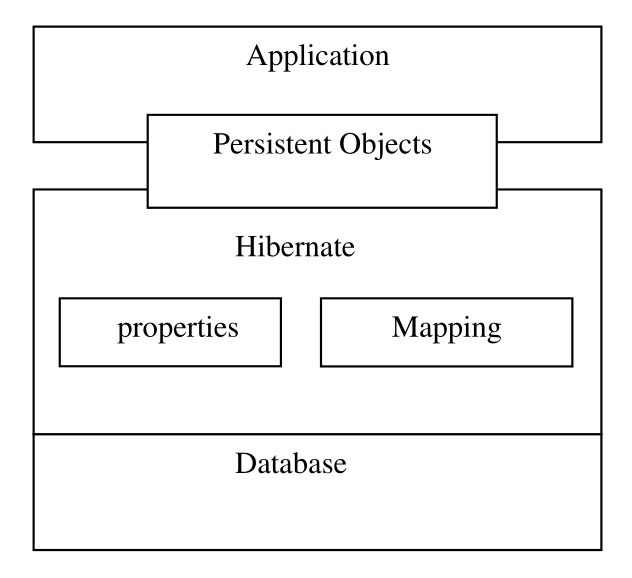
\includegraphics[width=0.6\textwidth]{hibernate.png}
  \caption{Hibernate工作原理(图标题:五号,宋体,段前段后6磅,行间距1.5)}\label{fig:hibernate}
  \vspace{\baselineskip}
\end{figure}
\clearpage

\section{XXX(3 级标题,四号,宋体,加粗,段前 6 磅,1.5 倍行距,建议不使用四级或更高级别目录、标题)}
\begin{table}
  \centering
  \caption{数据库表清单(五号,宋体,段前段后6磅,行间距1.5)}
  \label{fig:list}
  \begin{tabular}{cll}
    \toprule  %添加表格头部粗线
    \textbf{序号} & \textbf{名称}     & \textbf{说明} \\
    \midrule  %添加表格中横线
    1           & Project         & 项目表         \\
    2           & ProjectCategory & 项目分类表       \\
    3           & AppCategory     & 申报分类表       \\
    4           & MidChk          & 中期检查表       \\
    5           & CheckProject    & 项目中期检查表     \\
    6           & PassedProject   & 立项表         \\
    7           & Purview         & 权限表         \\
    8           & News            & 通知与指南表      \\
    \bottomrule %添加表格底部粗线
  \end{tabular}
\end{table}

\chapter{总结}
\section{完成的工作}
本文完成的主要工作:……

\section{存在的问题及下一步工作}
\chapter{引用参考文献}

参考文献应按文中引用出现的顺序列全,附于文末。
学位论文中列出的参考文献必须实事求是,论文中引用的必须列出,没引用的一律删去。
根据 GB 3469 规定,以单字母方式标识一下各种参考文献类型:

\begin{table}[htp]
  \centering
  \begin{tabular}{cc}
    \toprule
    \textbf{参考文献类型} & \textbf{名称} \\
    \midrule
    专著              & M           \\
    论文集             & C           \\
    析出论文            & A           \\
    报纸文章            & N           \\
    期刊文章            & J           \\
    学位论文            & D           \\
    报告              & R           \\
    标准              & S           \\
    专利              & P           \\
    其他文献            & Z           \\
    \bottomrule
  \end{tabular}
\end{table}

对于数据库,计算机程序及光盘图书等电子文献类型的参考文献,以下列字母为标识:
\begin{table}[htp]
  \centering
  \begin{tabular}{cccc}
    \toprule
    \textbf{参考文献类型} & \textbf{文献类型标识} \\
    \midrule
    数据库(网上)         & DB (DB/OL)      \\
    计算机程序(磁盘)       & CP (CP/DK)      \\
    光盘图书            & M/CD            \\
    \bottomrule
  \end{tabular}
\end{table}

测试引用:
\cite{zhangkun1994}
\cite{zhukezhen1973}
\cite{dupont1974bone}
\cite{zhengkaiqing1987}
\cite{jiangxizhou1980}
\cite{jianduju1994}
\cite{merkt1995rotational}
\cite{mellinger1996laser}
\cite{bixon1996dynamics}
\cite{mahui1995}
\cite{carlson1981two}
\cite{taylor1983scanning}
\cite{taylor1981study}
\cite{shimizu1983laser}
\cite{atkinson1982experimental}
\cite{kusch1975perturbations}
\cite{guangxi1993} \\
\cite{huosini1989guwu}
\cite{wangfuzhi1865songlun}
\cite{zhaoyaodong1998xinshidai}
\cite{biaozhunhua2002tushu}
\cite{chubanzhuanye2004}
\cite{who1970factors}
\cite{peebles2001probability}
\cite{baishunong1998zhiwu}
\cite{weinstein1974pathogenic}
\cite{hanjiren1985lun}
\cite{dizhi1936dizhi}
\cite{tushuguan1957tushuguanxue}
\cite{aaas1883science}
\cite{fugang2000fengsha}
\cite{xiaoyu2001chubanye}
\cite{oclc2000about}
\cite{scitor2000project}


%%%%%% 参考文献 %%%%%%
\backmatter
\bibliography{bib.bib}


%%%%%% 致谢 %%%%%%
\chapter{致谢(居中,小二,宋体,加粗,段前段后 18 磅,1.5 倍间距)}
对给予各类资助、指导、和协助完成研究工作,以及提供各种条件的单位及个人表示感谢。
致谢应实事求是,切忌浮夸与庸俗之词。
(小四,宋体,段前段后 0 磅,1.5 倍行间距)


%%%%%% 附录 %%%%%%
\appendix
\chapter{附录(小二,黑体,居中,加粗,段前段后 18 磅,1.5倍间距)}
 {%
  % 各个附录应添加进主目录,但不显示页码
  \ctexset{ section = { name = {附录}, number = \arabic{section} } }
\titlecontents{section}[5em]{}{\contentslabel{3.5em}}{}{}
\section{毕业设计文献综述}
\section{毕业设计开题报告}
\section{毕业设计外文翻译(中文译文与外文原文)}

主要列入正文内过分冗长的公式推导;
以备查读方便所需的辅助性数学工具或表格;
重复性数据图表、程序全文及说明。
论文的附录顺次为附录 1,附录 2……标号。
附录中的图和公式另编排序号,与正文分开。
}
\end{document}
